\documentclass[border=3pt]{standalone}
% Preâmbulo compartilhado pelos diagramas TikZ da aula 5 de IHC (Processos de Design)
\usepackage[T1]{fontenc}
\usepackage[utf8]{inputenc}
\usepackage{lmodern}
\usepackage{amsmath}
\usepackage{xcolor}
\usepackage{tikz}
\usetikzlibrary{arrows.meta,angles,quotes,decorations.pathmorphing,calc,
                positioning,shapes.geometric,shapes.misc,backgrounds,fit,
                math}

% Paleta (mesma dos SVGs originais)
% Paleta da disciplina de IHC: acento roxo (#755099), da capa do livro.
% (o nome "dblue" é mantido para não alterar todos os diagramas)
\definecolor{dblue}{HTML}{755099}
\definecolor{dorange}{HTML}{B3541E}
\definecolor{dgreen}{HTML}{4A7C59}
\definecolor{dred}{HTML}{9C4B4B}
\definecolor{dcream}{HTML}{F4F1EA}
\definecolor{dshade}{HTML}{DDD7C9}

% Função gaussiana (não normalizada por padrão de escala visual)
\pgfmathdeclarefunction{gauss}{3}{%
  \pgfmathparse{1/(#3*sqrt(2*pi))*exp(-((#1-#2)^2)/(2*#3^2))}%
}

% Estilos comuns (prefixo d... para não colidir com chaves internas do pgf)
\tikzset{
  >={Stealth[length=2mm]},
  dguide/.style={gray!55, dashed, line width=0.4pt},
  daxis/.style={gray!60, line width=0.7pt, ->},
  dbody/.style={fill=black!3, draw=black!80, line width=1pt},
  dacc/.style={draw=dblue, line width=1pt},
  dlbl/.style={black!55, font=\small},
  dsub/.style={black!45, font=\footnotesize},
  dstate/.style={circle, draw=black!80, fill=dcream, line width=1pt,
                 minimum size=17mm, font=\large, inner sep=1pt},
  dobs/.style={circle, draw=black!80, fill=dshade, line width=1pt,
               minimum size=14mm, font=\large, inner sep=1pt},
  dbox/.style={rounded corners=2pt, draw=black!80, fill=dcream, line width=1pt,
               align=center, inner sep=6pt},
  dop/.style={circle, draw=black!80, fill=white, line width=1pt,
              minimum size=6mm, inner sep=0pt, font=\small},
  dtrans/.style={->, dblue, line width=1pt},
  dmeas/.style={->, dorange, line width=1pt},
  dcurve/.style={line width=1pt, dblue},
  dcurveb/.style={line width=1.4pt, dorange},
}

\begin{document}
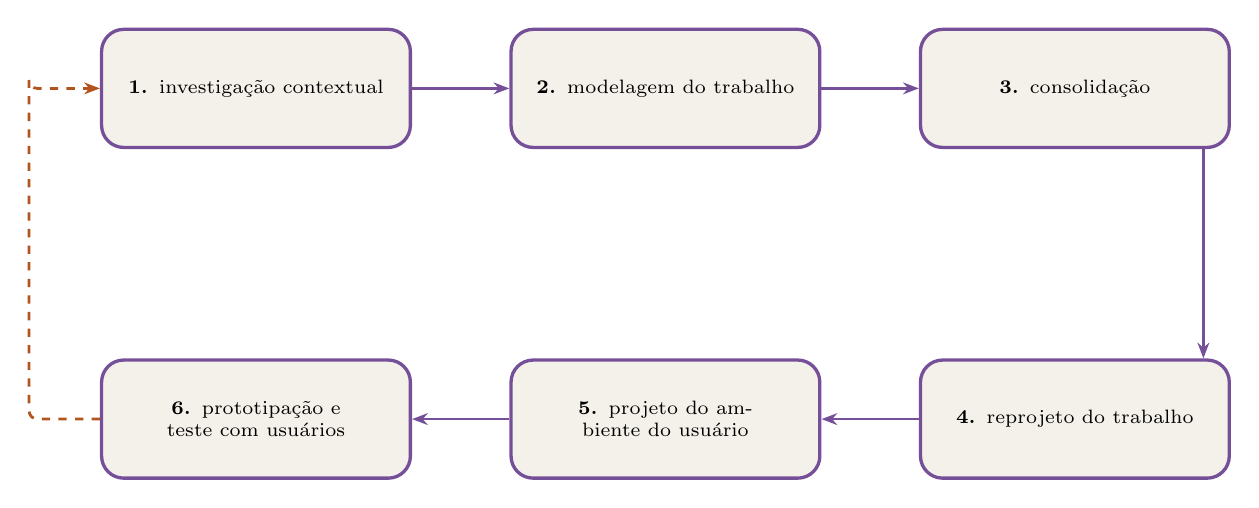
\begin{tikzpicture}[x=1cm,y=1cm,
   act/.style={dbox, rounded corners=8pt, text width=3.5cm, minimum height=1.5cm, font=\scriptsize, draw=dblue, line width=1.2pt},
   art/.style={text width=3.6cm, align=center, font=\tiny, dsub}]

  \node[act] (a1) at (0,0)  {\textbf{1.} investigação contextual};
  \node[act] (a2) at (5.2,0) {\textbf{2.} modelagem do trabalho};
  \node[act] (a3) at (10.4,0) {\textbf{3.} consolidação};
  \node[act] (a4) at (10.4,-4.2) {\textbf{4.} reprojeto do trabalho};
  \node[act] (a5) at (5.2,-4.2) {\textbf{5.} projeto do ambiente do usuário};
  \node[act] (a6) at (0,-4.2) {\textbf{6.} prototipação e teste com usuários};

  \draw[dtrans] (a1) -- (a2); \draw[dtrans] (a2) -- (a3); \draw[dtrans] ($(a3.south east)+(-0.35,0)$) -- ($(a4.north east)+(-0.35,0)$);
  \draw[dtrans] (a4) -- (a5); \draw[dtrans] (a5) -- (a6);
  \draw[dmeas, dashed, rounded corners=3pt] (a6.west) -- ++(-0.9,0) |- ++(0,4.2) -- (a1.west);


\end{tikzpicture}
\end{document}
